\documentclass[border=4pt]{standalone}
\usepackage{amsmath,amssymb,tikz}
\usetikzlibrary{arrows.meta,calc,decorations.markings}
\begin{document}
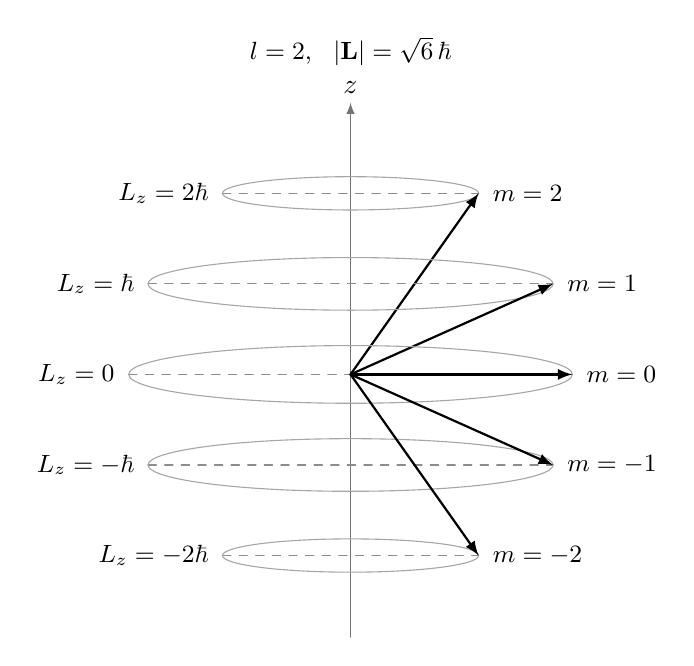
\begin{tikzpicture}[scale=1.15,>=latex,line cap=round]
  \draw[->,black!55] (0,-2.9) -- (0,3.0) node[above,black]{$z$};
  \pgfmathsetmacro{\L}{sqrt(6)}
  \foreach \m in {2,1,0,-1,-2}{
    \pgfmathsetmacro{\r}{sqrt(6-\m*\m)}
    \draw[dashed,black!45] (-\r,\m) -- (\r,\m);
    \draw[black!35] (0,\m) ellipse ({\r} and {0.13*\r});
    \draw[->,thick] (0,0) -- (\r,\m);
    \node[right,font=\small] at (\r+0.05,\m) {$m=\m$};
    \node[left,font=\small] at (-\r-0.05,\m) {$L_z=\ifnum\m=0 0\else\ifnum\m=1 \hbar\else\ifnum\m=-1 -\hbar\else\m\hbar\fi\fi\fi$};
  }
  
  \node[font=\small,anchor=south] at (0,3.3) {$l=2,\ \ |\mathbf L| = \sqrt{6}\,\hbar$};
\end{tikzpicture}
\end{document}
